\chapter{Testing the system}\label{chap:testing-the-system}
Testing the system is necessary to ensure quality.
In the following chapter we give an introduction to testing, and then describe and give examples of our approach to testing.
We will discuss unit testing, integration testing, formal reviews and mutation testing.
Finally we conduct a usability test of the system and examine the results.
\section{Introduction to testing}
Testing a system is a major part of software development and is a way to ensure that the system works as intended \cite{SoftwareTesting}.
In this chapter, we will take a look at what it means to test a system, different ways of doing it and why you should the system in the first place.

Testing can be split into two categories: Black-box testing and white-box testing. Both of these categories can be further split into static and dynamic testing.
When talking about black-box testing, it refers to testing the product without having access to the code itself as opposed to white-box where the tester knows the details of how the software works \cite{SoftwareTesting}.
The other terms used, static and dynamic testing refer to whether the tests are done while executing the code or not.
Static testing refers to testing something that is not running. For black-box testing this is usually related to reviewing the specifications, conducting tests where the testers pretend to be the customer, research standards for how to develop the system or compare it to similar software.
On a lower level, it also includes checking if the requirements specified for the project are possible to evaluate \cite{ToVSlides1}.
An example could be to check if the requirements contain sentences like "the system must be fast and cheap", which is not a directly measurable requirement.
Dynamic black-box testing on the other hand is the act of testing the executed system without looking at the code itself. This refers to manually testing the system by using it. It is usually done by intentionally trying to break the system by thinking like either a dumb user or a hacker \cite{SoftwareTesting}.

For white-box testing, static testing refers to testing in the form of pair programming, code reviews, walkthroughs.
All of those are ways of evaluating and testing at the code without running it.
Dynamic white-box testing on the other hand is related to testing the code where you know how it works. With this knowledge, it is possible for the tester to see some possible ways to break the system, that may not have been obvious otherwise, such as being able to see that given a specific input, the system will throw a divide by zero exception and crash the system \cite{ToVSlides1}.
Other parts of dynamic white-box testing include unit testing and looking at coverage measures, which we will dive further into in this chapter.

\section{Unit testing}
Unit testing is our primary way of testing our system, and belongs in the dynamic white-box testing category.
The purpose of unit testing is to see if an isolated subset of the system works as expected, given some pre-defined input \cite{TestDrivenDevelopment}.
For this project, unit tests are utilized for both the React frontend and the API, to ensure that the system works as intended.

\subsection{Choice of framework}
One of the first decisions when creating unit tests, is the choice of test runner.
Since the React library is shipped with Jest \cite{ReactRunningTests}, and since both parts of the system are JavaScript based, it seemed like the optimal solution to use the same test runner.
However, after using Jest for testing the API for a while, several issues surfaced when trying to implement mock functions related to our ORM and some TypeScript functionality in general.
To simplify the creation of unit testing on the API, the test driver for this was changed to Mocha.

One of the main differences between Jest and Mocha is that Jest is a complete suit that supports running the tests, asserting results, stubbing, test coverage and much more.
Mocha, on the other hand, is just a test runner and requires additional libraries for asserting, stubbing and generating code coverage results \cite{Mocha}.
We chose to use Chai for assertions, Sinon for stubbing and Nyc for generating code coverage.

\subsection{What to test}
The answer to what should be tested varies a lot between the frontend and the API.
One of the axioms of testing states that it is impossible to test a program completely, and should be seen as a risk-based exercise where the tester asserts which parts of the system should be tested, and how thoroughly it should be tested \cite{SoftwareTesting}.
For the frontend of the system, it would be possible to test whether each component is rendered to the user, if all the information is correct, what happens if you use 0 as input to the function, 1 as input, 3 as input.. And so on.
Instead, we chose to focus on testing if the components that are conditionally rendered are shown when the conditions are fulfilled.
An example of this could be the \textit{Show User} page, where the system should show tutor info if and only if the user is actually a tutor.
This now leads to test cases like is the info rendered if:
\begin{itemize}
    \item the user is a tutor?
    \item the user is a tutor?
    \item the user is a tutor, but the tutor information is invalid?
    \item the user is a tutor, but the tutor information is incomplete?
\end{itemize}

In addition to the conditional rendering, any business logic located on the frontend should be tested to ensure both that it works as intended, but also to ensure that any future updates to the code will not break it, which is referred to as regression testing.

For the API, some functionality like the ORM is handled by external packages. Since this is not code we're writing ourselves, we have chosen to assume that the developers of the packages have tested the software and we will not have to.
We focus on unit testing our controllers and middleware to ensure that they work as expected, and instead do some integration testing for the external packages, to ensure that they work as expected when integrated into our system. This will be further described in \autoref{sec:integrationTesting}.

\subsection{Stubbing}
A major obstacle for generating our tests was to avoid the calls to the ORM in the API, which would connect to the database.
At first, we considered different ways to handle this connection, such as having a test database that would be wiped before each test to generate a controlled environment.
However, after doing more research we realized that instead of connecting to a real world configuration, it would be beneficial to be able to control exactly which values should be returned.
This principle is called stubbing \cite{SoftwareTesting}.
The idea is that instead of calling a given function, we create a stub function that is called instead.
An example of this can be seen in the unit test in \autoref{lst:unitTestStubbing}, where we stub the function call to \texttt{getByEmail} in the \texttt{userService}.
In the real code, the code seen on \autoref{lst:getByEmail} would be called as a part of the call to the login function on line 16, which connects to the database, but instead of doing so we use the Sinon library to stub the function, and tell it to instead throw an exception, so we can see how the controller handles this case.

\begin{lstlisting}[caption={Unit test with stubbing},label={lst:unitTestStubbing}]
...
it('returns status 400 if service throws exception', async function() {
    const request = {
        body: {},
    };
    const req = mockReq(request);

    const res = mockRes({
        status: function(s: number) {
            this.statusCode = s;
            return this;
        },
    });
    const stubResult = sinon.stub(userService, 'getByEmail').throws('exception');

    await AuthController.login(req, res);
    expect(res.statusCode).to.equal(400);
    stubResult.restore();
});
...
\end{lstlisting}

\begin{lstlisting}[caption={Actual getByEmail function},label={lst:getByEmail}]
static getByEmail = async (email: string): Promise<User> => {
    //Get user from database
    const userRepository: Repository<User> = getRepository(User);
    return await userRepository.findOneOrFail({ where: { email } });
};
\end{lstlisting}

As seen on \autoref{lst:unitTestStubbing} lines 3 to 13, we also made use of mocking for defining the request and response parameters used for requests to the controller.
This allows us to check whether the correct status code is returned from the controller by overriding the status function.
Normally, the function would set the headers that are returned to the client requesting the API.
However, for this test we are only interested in seeing which parameter the status function is called with to ensure that it matches our expectations.
This way it is now possible to check if the \texttt{statusCode} property on the response is set to what we expect, as seen on line 17.

Finally, the stub is restored to make sure that it only behaves in this limited way in the scope of the unit test.

\subsection{Metrics of good testing}
There are multiple ways of measuring whether the created unit tests are sufficient.
Our primary metric for our automated tests are code coverage, which measures how much of the code base is covered by unit tests.
This is split into four categories: Statement coverage, branch coverage, function coverage and line coverage.

\begin{figure}[H]
    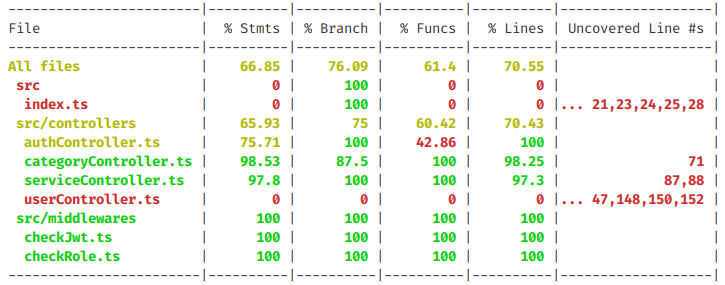
\includegraphics[width=\linewidth]{/test.png}
     \caption{The output of the code coverage reporter NYC}
     \label{fig:testResults}
 \end{figure}

We used a configuration to report files with 0-50\% coverage as red, 50-75\% as yellow and 75-100\% as green.
While this is a good indicator about how much of the code has been tested, it does not ensure that the tests are useful and correct.

To ensure this, we make use of formal reviews of both the code and tests.

\section{Integration testing}\label{sec:integrationTesting}
While unit testing is great for testing if a given module works in isolation, it is just as important to test if module A and B can work together as intended.
This is where integration testing comes in. 
Integration testing is an incremental process where an increasing amount of modules are put together and every time this happens the new and larger group is tested.
Integration testing is similar to unit testing, but it is a higher level of testing where we do not worry about the isolated functionality of the modules.
It is also common to use external libraries or module that are not necessarily developed by ourselves and it is therefor important to perform integration tests to make sure that the introduction of external module did not introduce any new bugs, or unexpected behavior. 

In this project, integration testing was been done in the API to verify that the external libraries added via the node package manager work as intended.
An example of an external library that was tested with integration testing is the \texttt{class-validator} package, where we give it a model that is intentionally wrong to see if it returns the data in the way we expect.
We can then continue on testing the controller where the validator is called, to see if it behaves as expected in case the class validator works.
This kind of testing can also be used for regression testing, as we will be made aware if the behavior of the validator changes due to the test failing.

\section{Formal review}
To ensure the quality of the code and the correctness of the tests, we made use of formal reviews.
A formal review is a process that belongs to the static white-box testing category.
A formal review contains four essential elements \cite{SoftwareTesting}:
\begin{itemize}\label{formalreview}
    \item Identify problems
    \item Follow rules
    \item Prepare
    \item Write a report
\end{itemize}
The goal of the review is to find problems or deficiencies in the software, with criticism directed at the design or the code itself.
Rules should be established regarding the process, such that they can be followed during a formal review.
An example of a rule could be defining the maximum amount of code to be reviewed at one time, or how many reviewers should examine the code.
Each participant in the review should be prepared for it, such that they can contribute.
Depending on the type of review, the participants could have different roles, and this should be known before the review begins, such that the roles can be actively fulfilled.
The review group should ultimately produce a report summarizing the results of the review, such that other developers can become aware of the results. 

\subsection{Our formal review process}
Initially when reviewing our code we would have two reviewers individually review the code and write comments and suggested changes. 
This would be done by creating a pull request (PR) to the develop branch and the author would then assign two reviewers.
When a review had been submitted by the reviewer, the author would go through the list of suggested changes to the code and fix the code or ask clarifying questions to the reviewer.
After two reviewers had accepted the PR it could be merged to the develop branch. 
\\\\
To further ensure that the quality of the code that is pushed to develop is of acceptable quality we use continuous integration (CI).
The CI ensures that the project is able to build without any errors, and that the unit tests succeed. 
That way we can be sure that the develop branch is never a broken build.
Additionally we use a linter that we can configure to test that the code follows some rules and coding standards. 
We also make the CI run the linter, and if the code does not follow the standards set it will fail to built.
\begin{figure}[H]
    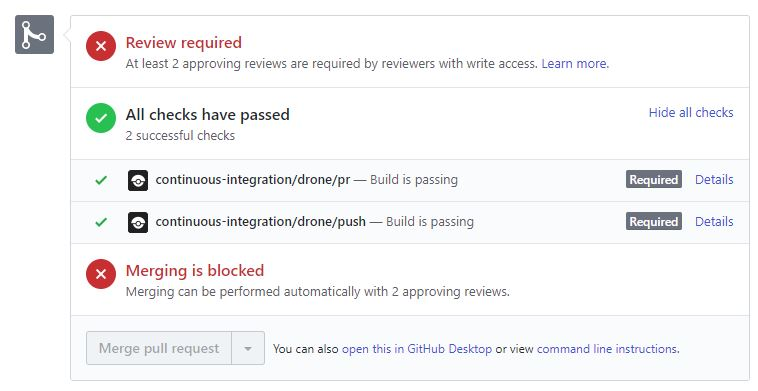
\includegraphics[width=\linewidth]{/ci.JPG}
    \caption{The CI has to be able to build for a PR to be merged}
    \label{fig:continous-integration}
\end{figure}
\noindent
During the later stages of the project we decided to change our approach to formal reviews.
Rather than have two developers individually review a PR, we strove to have the developers get together for the review.
This would ensure more discussions arose based on the PR, and increase the overall quality of the review.
\\\\
In terms of the four essential elements defined in \autoref{formalreview}, our process achieves these elements.
We did not directly write a report, as this element is mostly necessary for larger systems developed by larger teams.
Instead, the results of our reviews were made available through comments and suggestions to the PRs, such that other developers could access them.
\begin{figure}[H]
    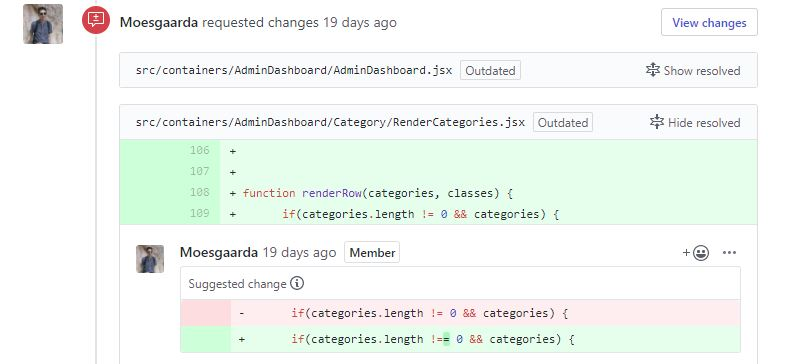
\includegraphics[width=\linewidth]{/commentonpr.JPG}
    \caption{An example of a comment on a PR}
    \label{fig:comment-on-pr}
\end{figure}

\section{Mutation testing}
Even with a code coverage of 100\%, the traditional test coverage measures only show how much of the code is executed by the tests, and not whether the tests are able to detect faults in the code \cite{pitest}.
This means that it is possible to get a full line, statement, and branch coverage by simply executing the code without any useful assertions in the test suite.
One way to combat this problem is with the use of mutation testing.
The idea behind mutation testing is to run some automated software (the mutation testing system), which will generate mutants by modifying minor parts of the system such as replacing a less than check with a greater than check.
The objective is to have a test suite that \textit{kills} the mutants by revealing that the mutant behavior differs from the original program \cite{mutationtesting}.

Mutation testing can be split into two categories: strong and weak mutations.
In strong mutation, we are only interested in the external observation of the code, meaning that the produced output of a given function is different when the mutation is introduced \cite{mutationtesting}.
These mutants can be hard to kill, since the effect of the mutant can be lost before the program terminates.
To be able to do a deeper check, we introduce weak mutation, where we define a mutant as killed if it leads to different results after \textit{some} execution, rather than after all code has finished executing.
Weak mutation testing is usually preferable to strong mutation testing in safety-critical systems, since it will be able to find more potential bugs, but with the tradeoff that execution time of the mutation analysis will increase.

After running the mutation test, the framework will generate a mutation score based on the percentage of mutants killed.
This can now be used to improve the test suite, by creating new test cases until all mutants can be killed.

\section{Usability testing}
Opposed to the previously mentioned tests, usability testing is not directly focused on the functionality and structure of the code, but rather how easy the system is to use by real users.
Even though the system may seem exceedingly simply to use by the developers, this is rarely the case for the actual users.
To increase the usability of the system during the development, the development team can make use of the personas defined in \autoref{sec:personas} during the formal review.
The reviewers can subjectively evaluate the design choices made against the personas and try to conclude whether all the personas would be able to understand the system.

However, this does not solve the problem of the reviewers knowing how the system works, and can easily navigate through it due to their deep understanding of the system.

Instead, it will be beneficial to conduct usability testing, where the testers try out the system under observation.
The testers, in this case, are usually either potential users of the system, or other employees who have not been a part of developing the software, to get more reliable results \cite{SoftwareTesting}.
\\\\
With usability testing, it is possible to get feedback on more subjective parts of the system, such as the user interface and whether the errors displayed to the user are useful and understandable without having a degree in software engineering \cite{SoftwareTesting}.

When conducting usability tests, a set of pre-defined tasks are given to the testers one at a time.
These tests should aim to resemble how actual users would use the system, to observe where they struggle to understand how the system works.

\subsection{Our usability tests}
To get feedback on the subjective parts of the system, we conducted usability tests.
The tests that the users performed can be found in \autoref{app:usability}.

\subsubsection{Comparison of the tests}
\autoref{tab:usabilitytest} shows the different testers and the time it took for them to perform the tasks defined.
The tester called Mikkel encountered some issues with logging in.
This was caused by some issues related to the test setup, and resulted in the time spent on the first few assignments not being indicative of the actual time it would take.
While the time was invalid, he still completed the assignments, looking for design deficiencies.
\begin{table}[]
    \begin{tabular}{|l|l|l|l|l|}
    \hline
                                            & Mikkel     & Melanie      & Martin           & Robin               \\ \hline
    Create user                             & N/A        & 1 min 31 sec & 1 min 24 sec     & 1 minute 11 seconds \\ \hline
    Log in                                  & N/A        & 10 seconds   & 34 seconds       & 18 seconds          \\ \hline
    Change language                         & N/A        & 15 seconds   & 14 seconds       & 12 seconds          \\ \hline
    Find "Butterfly"                        & N/A        & 13 seconds   & 12 seconds       & 10 seconds          \\ \hline
    Find other services by "Mathias Møller" & N/A        & 12 seconds   & 1 min 31 seconds & 13 seconds          \\ \hline
    Delete user                             & N/A        & 20 seconds   & 21 seconds       & 22 seconds          \\ \hline
    Login as admin                          & N/A        & 20 seconds   & 22 seconds       & 18 seconds          \\ \hline
    Create a service                        & 21 seconds & 38 seconds   & 45 seconds       & 30 seconds          \\ \hline
    Rate specific service                   & 10 seconds & 19 seconds   & 20 seconds       & 21 seconds          \\ \hline
    Log out                                 & 5 seconds  & 10 seconds   & 4 seconds        & 5 seconds           \\ \hline
    \end{tabular}
    \caption{A comparison of the time it took to perform the different tasks}
    \label{tab:usabilitytest}
\end{table}
Creating a user consistently took the longest amount of time.
As can be seen, for all applicable tester, it took longer than 1 minute.
The reason for this is that when creating a user, more input is required than many other parts of the system.
The testers encountered an issue with their passwords, as the restrictions put on this made them have to redo this.
The password requires at least 8 characters, with one number and one capital character.
Another consistent issue was the design of choosing a language when creating a user.
The user has to choose the languages they are capable of speaking, such that, if they were to become tutors and create a service, prospective learners would know in which languages the service could be provided.
During the test it was implemented as a dropdown in which users could select multiple languages at a time.
This turned out to be unintuitive, as they were unsure whether or not they had actually chosen a language after selecting one.
This led to some of them repeatedly clicking the same language multiple times, selecting and deselecting it.
A possible fix for these issues could be to close the dropdown once a language has been chosen, but this might not communicate that the user is capable of selecting multiple languages.
\\\\
The assignment to find other services by a certain tutor had the largest deviation in terms of time spent.
Two of the testers spent respectively 12 and 13 seconds, while the third spent a full minute and 31 seconds to complete the task.
The reason for this deviation is that the tester was confused what exactly he was supposed to do.
Once he figured it out, he felt it was not immediately obvious where to go.
Finally, he attempted to search for the tutor, which ended in him encountering a bug in which the search functionality did not work.
This bug has since been fixed such that users can search for the name of a tutor.
\\\\
One of the testers commented on the icons used in the system, saying some of them might not be as intuitive as intended.
This tester was confused with the log in button, thinking it looked like a log out button instead.
Generally, the assignments felt easy to complete for the testers.
Outside of the two discussions above, the assignments were completed quickly, and the testers spent around the same amount of time on all of them.
This, along with the lack of problems caused by the design during testing could indicate that, generally, the design of the system is fairly intuitive, while some of the icons could be a bit unintuitive. 


